\chapter{Results}%Or Results
\label{ch:res}
Let us start drawing a big picture of the different topics that emerged after the latent ideology analysis. 


Fig \ref{fig:diptest} summarize the size of the newtorks and the diptest result, so the polarization, for each topic. The first thing to note is the fact that to the highest polarization corresponds the smaller topics, with the exception of topic 14. For the first two topics the polarization is significantly higher than the others.


\begin{figure}[H]
    \centering
    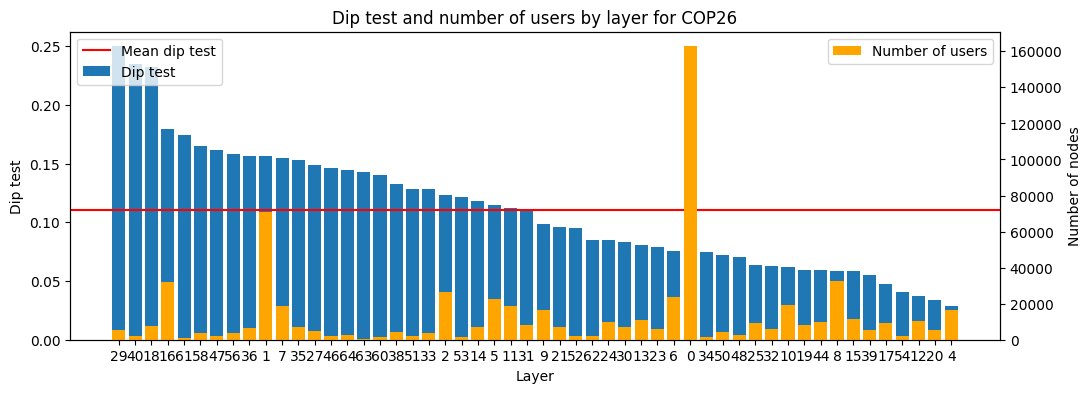
\includegraphics[width=0.95\linewidth]{Chapter5//figures/diptest_cop26.png}
    \caption{Dip test and number of users for cop26 topic by topic}
    \label{fig:diptest}
\end{figure}

\section{RQ1 Most Polarized Topics}


Fig \ref{fig:networks_polarization} let us visualize the most and the least polarized topics, every network represent the retweet network of the 100 biggest influencers, in the leftmost plot we can find the full network while in the rightmost only the influencers are present. In the most polarized topics we can clearly see how the influencers are almost equally split between the two poles. Falkenberg it its work identified a majority of pro climate and a minority of climate skeptics, but looking at a topic level we can see how the two groups are equally split, and the networks that present the majority-minority dicotomy are the least polarized. A notable example is the most polarized topic: "Canada Climate Change goals" which refers to the announcement of Canada's first minister to cap gas and oil emissions. This decision caused many disagreement, in Tab \ref{tab:canadatweets} some random tweets against the decision, user 1 argument that this will destroy the economy, user 2 instead is generally against all the decision of Trudeau, as states in her biograpahy : "Lover of gardening, antiques and anyone who wants to see the end of the Trudeau government." This  follows the typical elite polarization pattern, where political exponent strictly adhere to their party policies, in this case it is not a political party but a politically-aligned individual which is, in some way, forced to follow her self-imposed guidelines in her biography to avoid cognitive dissonance \cite{Festinger_dissonance_57}.

\begin{table}[]
\centering
\begin{tabular}{|p{1in}|p{4in}|}\hline
\textbf{user} & \textbf{tweet} \\ \hline
User1     & This meme could just as easily apply to Canada. Trudeau’s willingness to destroy our economy to the benefit of others is akin to cutting off our noses to spite our faces!\%. \\ \hline
user2        & \#COP26 Maybe some people are still fooled by Justin Trudeau and his dishonest climate change stories, but there are plenty of us here in Canada who are not. Look into the truth about the Lytton fire. It won't come out of Justin Trudeau's mouth \\ \hline
user3          & Capping emissions in the country while exporting oil, gas and coal out of the country. Hypocrisy.
 \\ \hline
\end{tabular}
\caption{}
\label{tab:canadatweets}
\end{table}




It is interesting to note in Fig \ref{fig:ridge_topics} the distribution of the tweets of each topics over time during the cop, the dotted line marks the start end end date of COP26. The most polarized had interest only in few days losing quickly the interest. The opposite happens in the least polarized topics where the discussion is distributed over a longest timespan.  



\begin{figure}[H]
    \centering
    \begin{minipage}{0.50\textwidth}
        \centering
         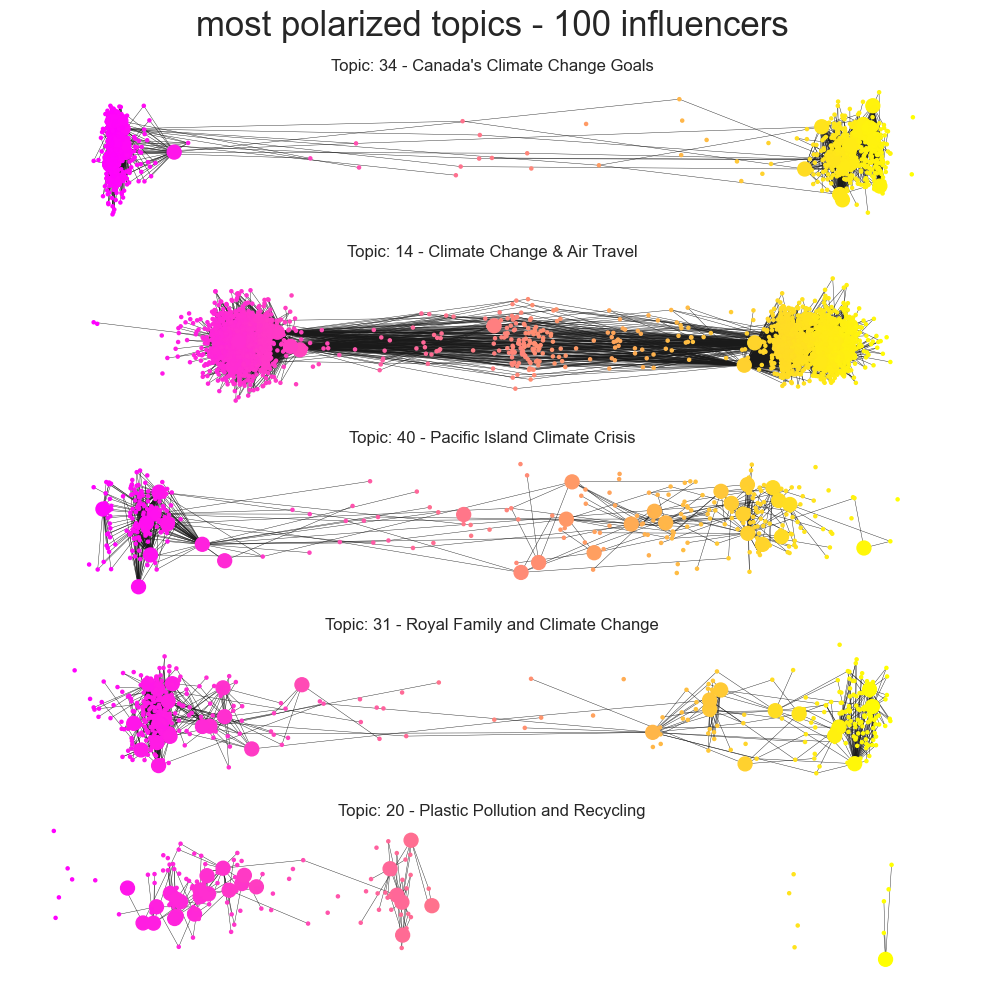
\includegraphics[width=0.98\linewidth]{Chapter5//figures/most_pol_cop26.png}
        \caption{most polarized topics}
    \end{minipage}\hfill
    \begin{minipage}{0.50\textwidth}
        \centering
         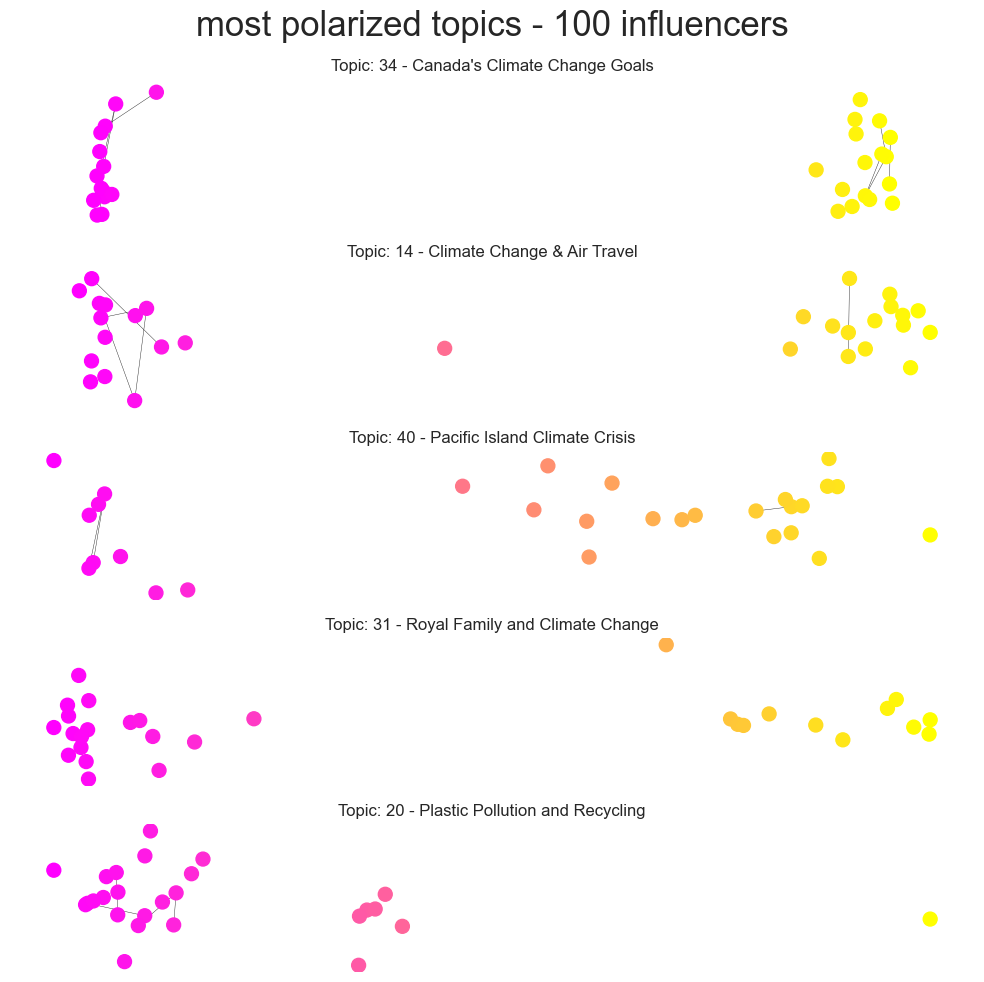
\includegraphics[width=0.98\linewidth]{Chapter5//figures/most_pol_cop26_inf.png}
        \caption{most polarized topics only infleuncers}
    \end{minipage}
    \begin{minipage}{0.50\textwidth}
        \centering
         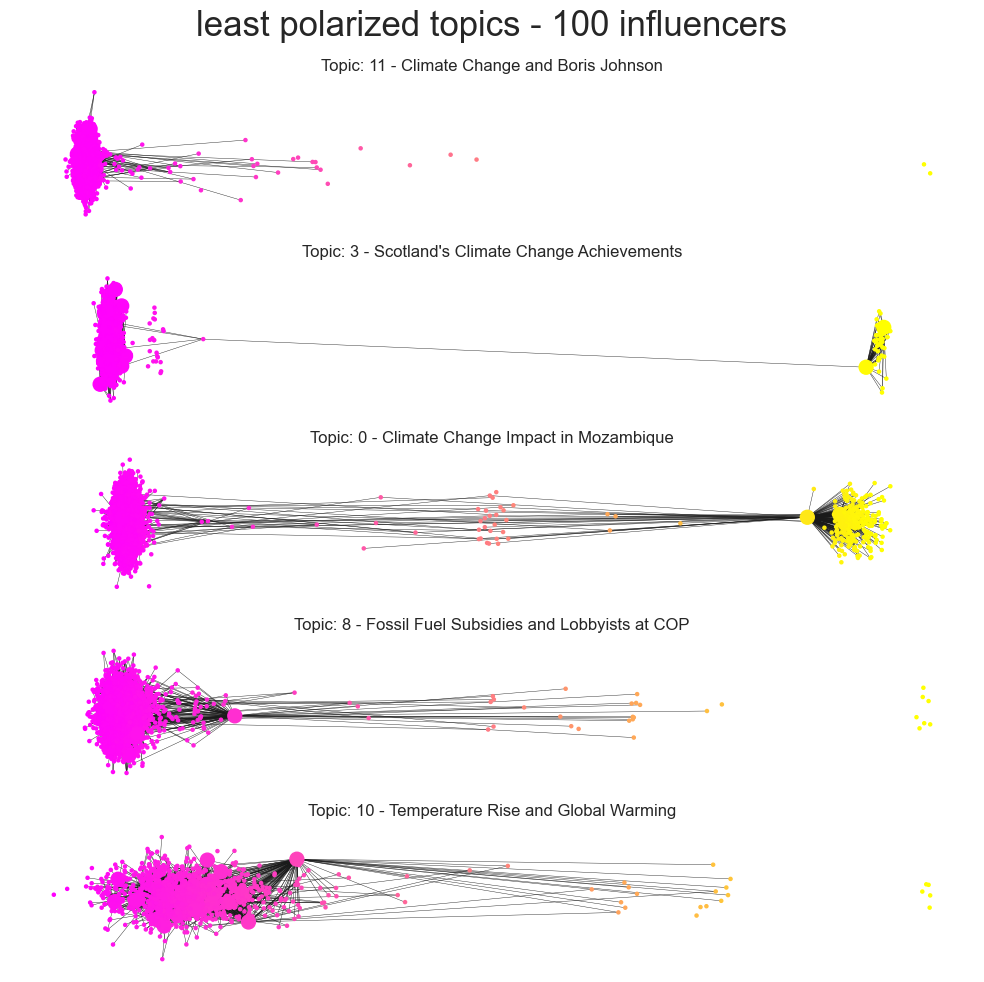
\includegraphics[width=0.98\linewidth]{Chapter5//figures/least_pol_cop26.png}
        \caption{least polarized topics}
    \end{minipage}\hfill
    \begin{minipage}{0.50\textwidth}
        \centering
         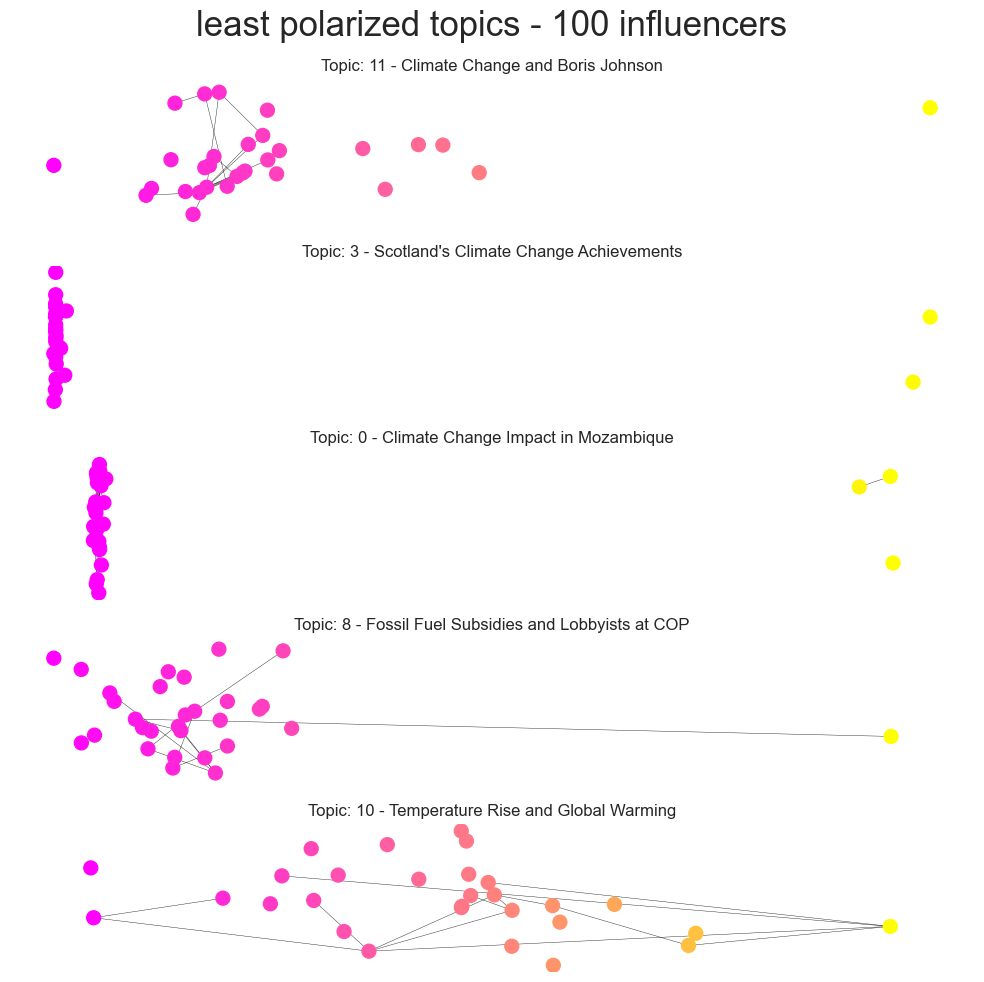
\includegraphics[width=0.98\linewidth]{Chapter5//figures/least_pol_cop26_inf.png}
        \caption{least polarized topics only influencers}
    \end{minipage}

    \caption{least and most polarized topics}
    \label{fig:networks_polarization}
\end{figure}


\begin{figure}[H]
    \centering
    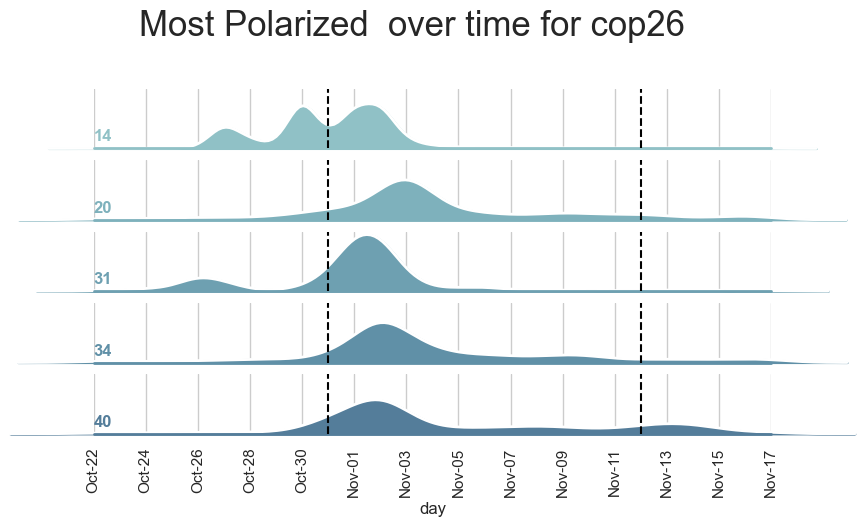
\includegraphics[width=0.75\linewidth]{Chapter5/figures/ridge_most_26.png}
     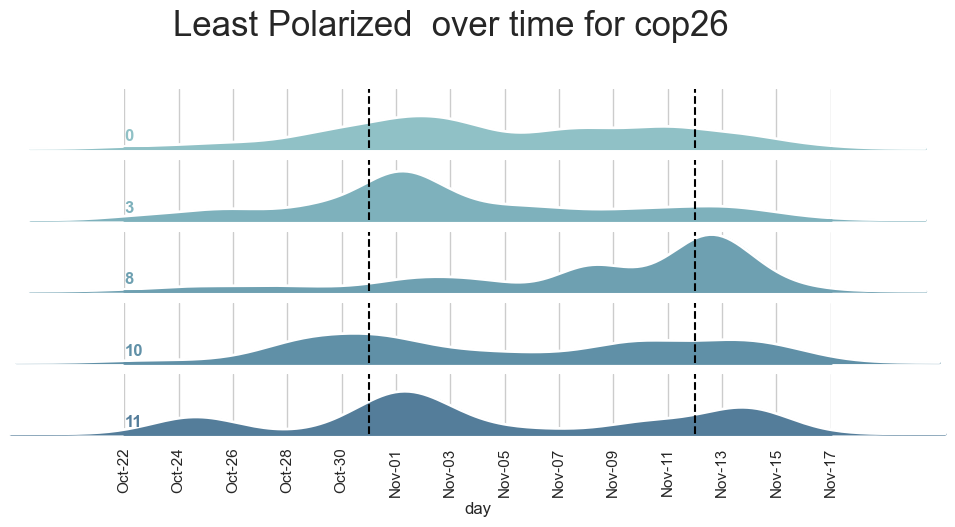
\includegraphics[width=0.75\linewidth]{Chapter5/figures/ridge_least_26.png}
    \caption{Enter Caption}
    \label{fig:ridge_topics}
\end{figure}


\section{RQ2 Longitudinal analysis}

In this section we compare the polarization between cop21 and cop26, to do so, we had to run the topic modeling together, in Fig \ref{fig:diptesto cop2x} the diptest results is shown, here we can find a similar trend of the cop26, the biggest topics are less polarized, with the exception of topic 9. Fig \ref{fig:2126_share} helps understanding the share of the tweets between cop21 and cop26. We can see how topic 9 which is the most polarized is composed mostly by tweets from cop26, which is aligned with the literature. Now we will look into some topics, creating the network if retweets both for bot COPs and we will compare them. We can compute this analysis only on topic 1,3 and 12 which are the ones that are polarized and have enough tweets in bot cops to run latent ideology.  

\begin{figure}[H]
    \centering
    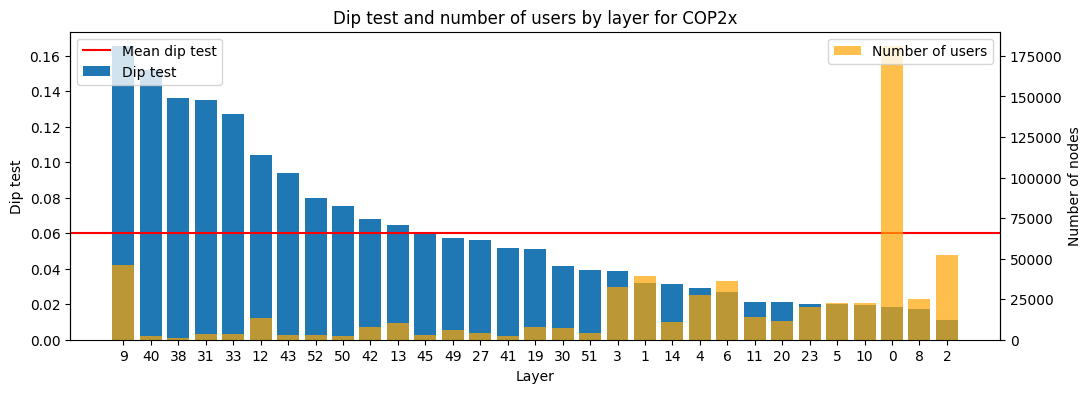
\includegraphics[width=0.8\linewidth]{Chapter5//figures/diptest_cop2x.png}
    \caption{Enter Caption}
    \label{fig:diptesto cop2x}
\end{figure}

\begin{figure}[H]
    \centering
    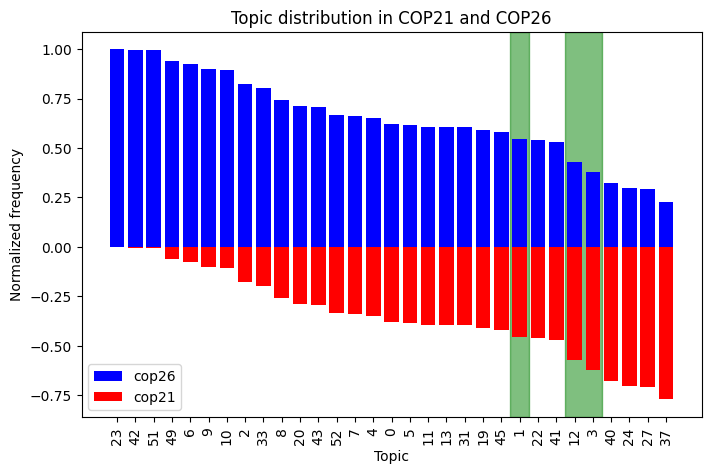
\includegraphics[width=0.8\linewidth]{Chapter5/figures/cop21vscop26.png}
    \caption{Enter Caption}
    \label{fig:2126_share}
\end{figure}

Fig \ref{fig:cop2x_network_comparison} show the results of this analysis. It is worth noting how topic 12 is the topic talking about Canadian fossil fuels, discussion that was present in both cops, but with a very different level of polarization. Overall the results confirm the hypotesis that cop26 is more polarized of cop21, but these are just three topics, to confirm this we should run the same analysis with more data.

\begin{figure}[H]
    \centering
    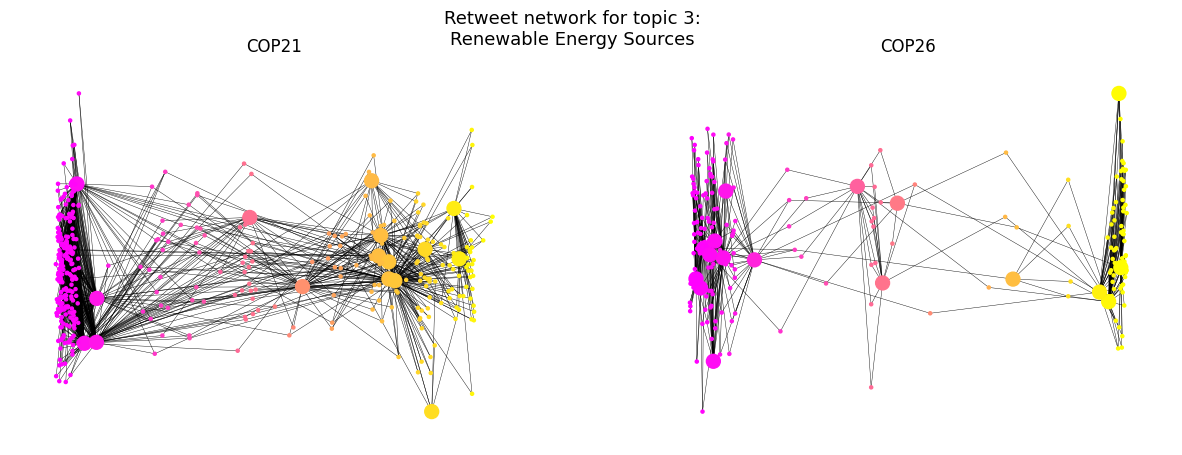
\includegraphics[width=0.95\linewidth]{Chapter5//figures/21vs26_t3.png}
    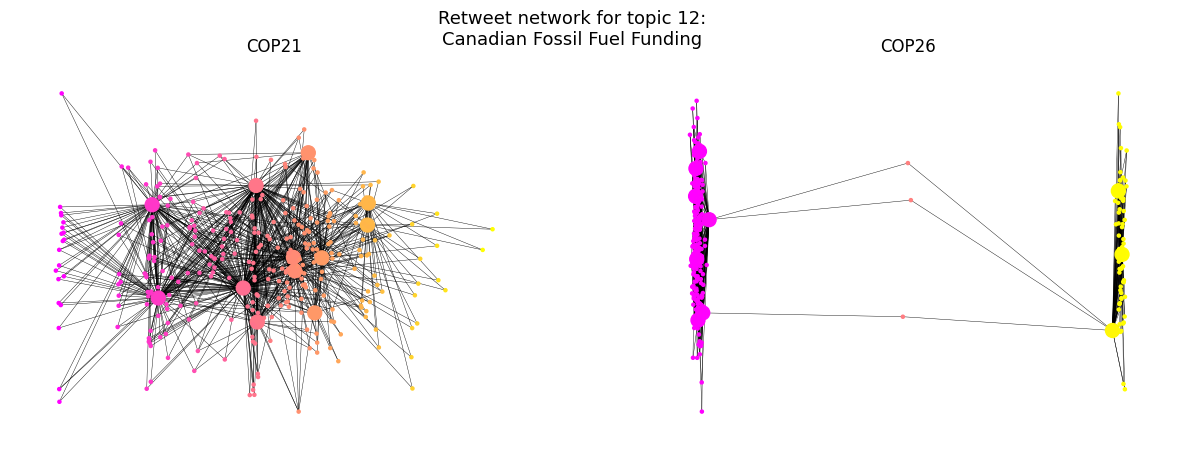
\includegraphics[width=0.95\linewidth]{Chapter5//figures/21vs26_t12.png}
    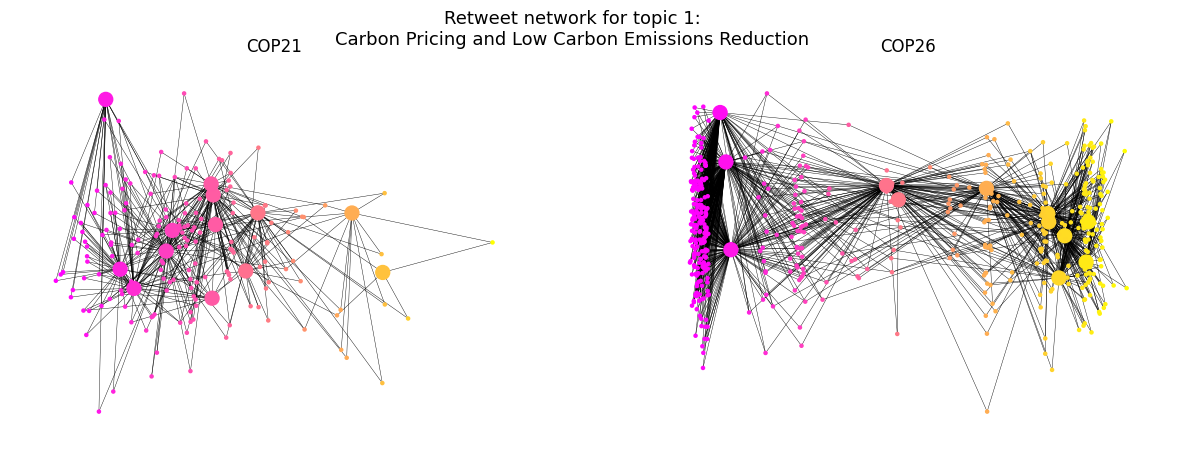
\includegraphics[width=0.95\linewidth]{Chapter5//figures/21vs26_t1.png}
    \caption{Enter Caption}
    \label{fig:cop2x_network_comparison}
\end{figure}

\section{RQ3 User polarization among different topics}
After computing the polarization score for all users we can now analyze whether the the users are polarized in the same way among all the topics they were active in.

The number of users involved in this analysis is 22161 active in 26 topics. most of them (16141) were only active in one topic, the maximum is 23 and the average is 1.53 topics per user. 

Then we computed, for each user present in more than 1 topic, the average and the standard deviation of the score. This value is higher for the users that are present in both side of the spectrum so this allow us to identify the degree to which users tend to be monopolar.

Fig \ref{fig:std_avg} show how the distribution of the average score for every topic aggregated together, this matches with the global results of Falkenberg, where a majority is present on the $-1$ side versus a minority in the $1$ side.

In the std we can see how there is a strong tendency to stay in the same side of the spectrum.

\begin{figure}[H]
    \centering
    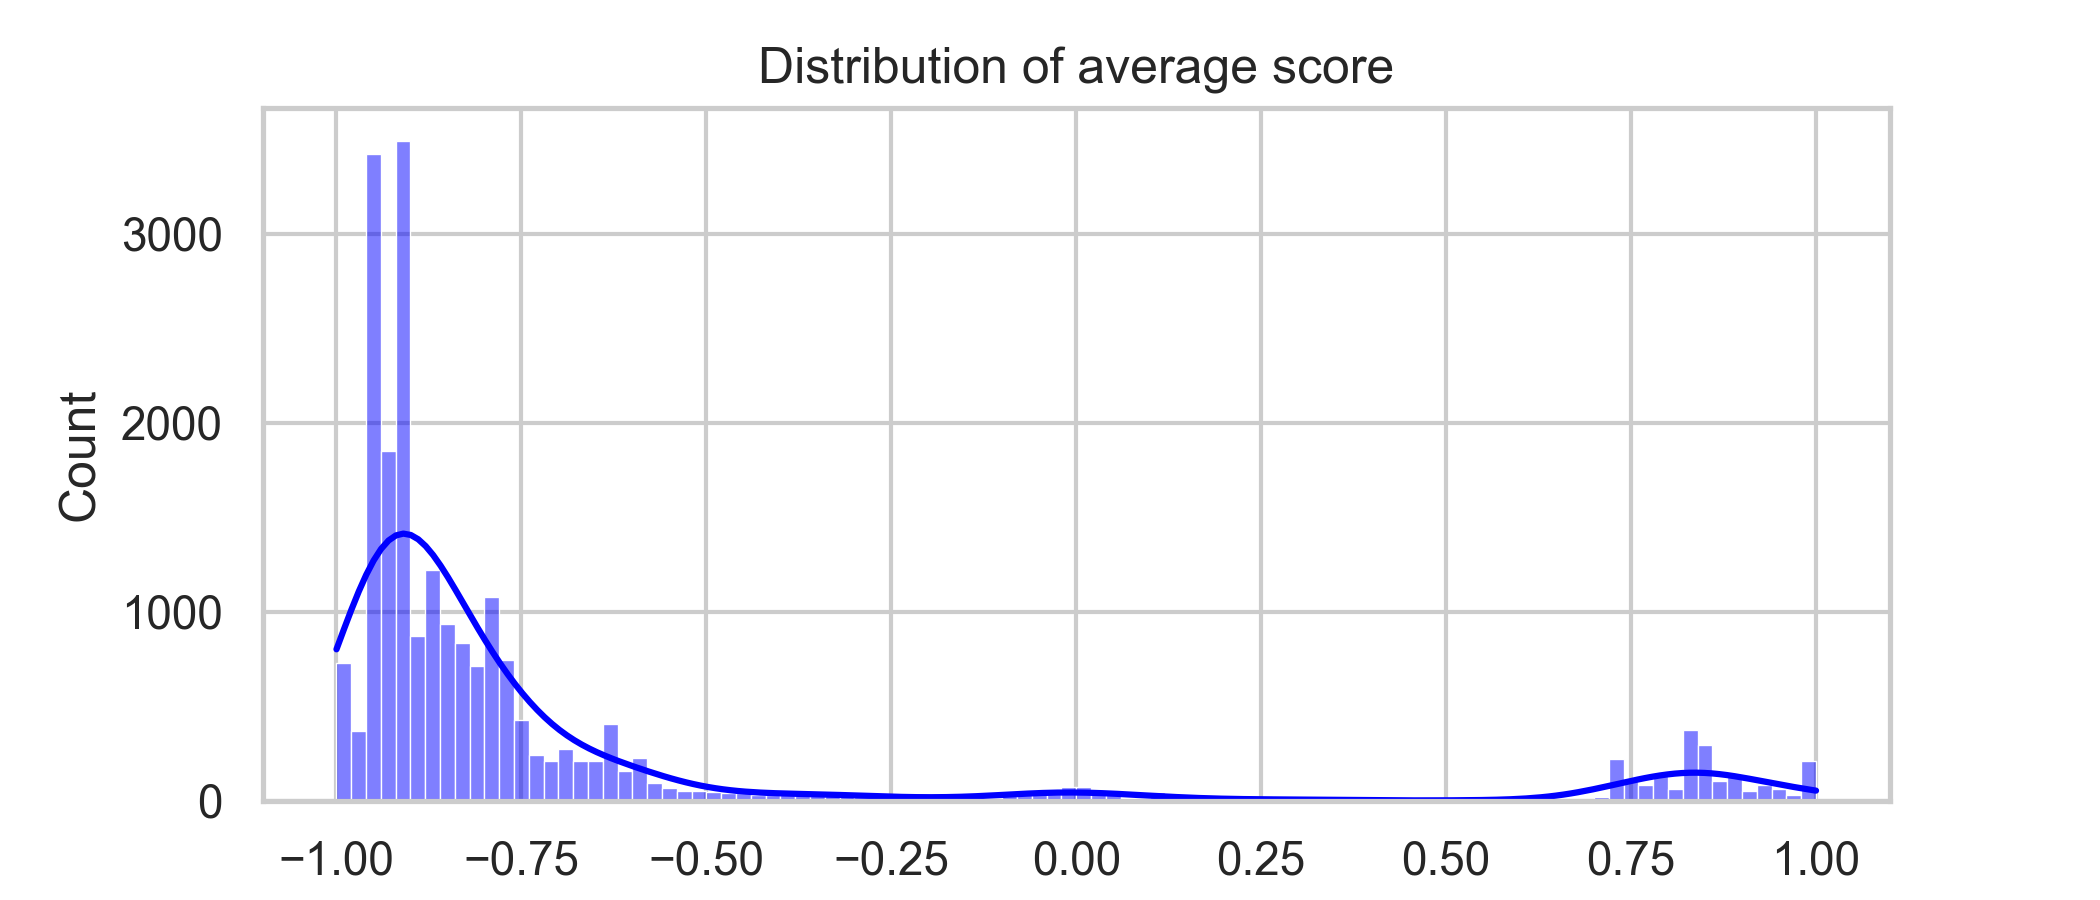
\includegraphics[width=0.9\linewidth]{Chapter5//figures/avg_score.png}
    
    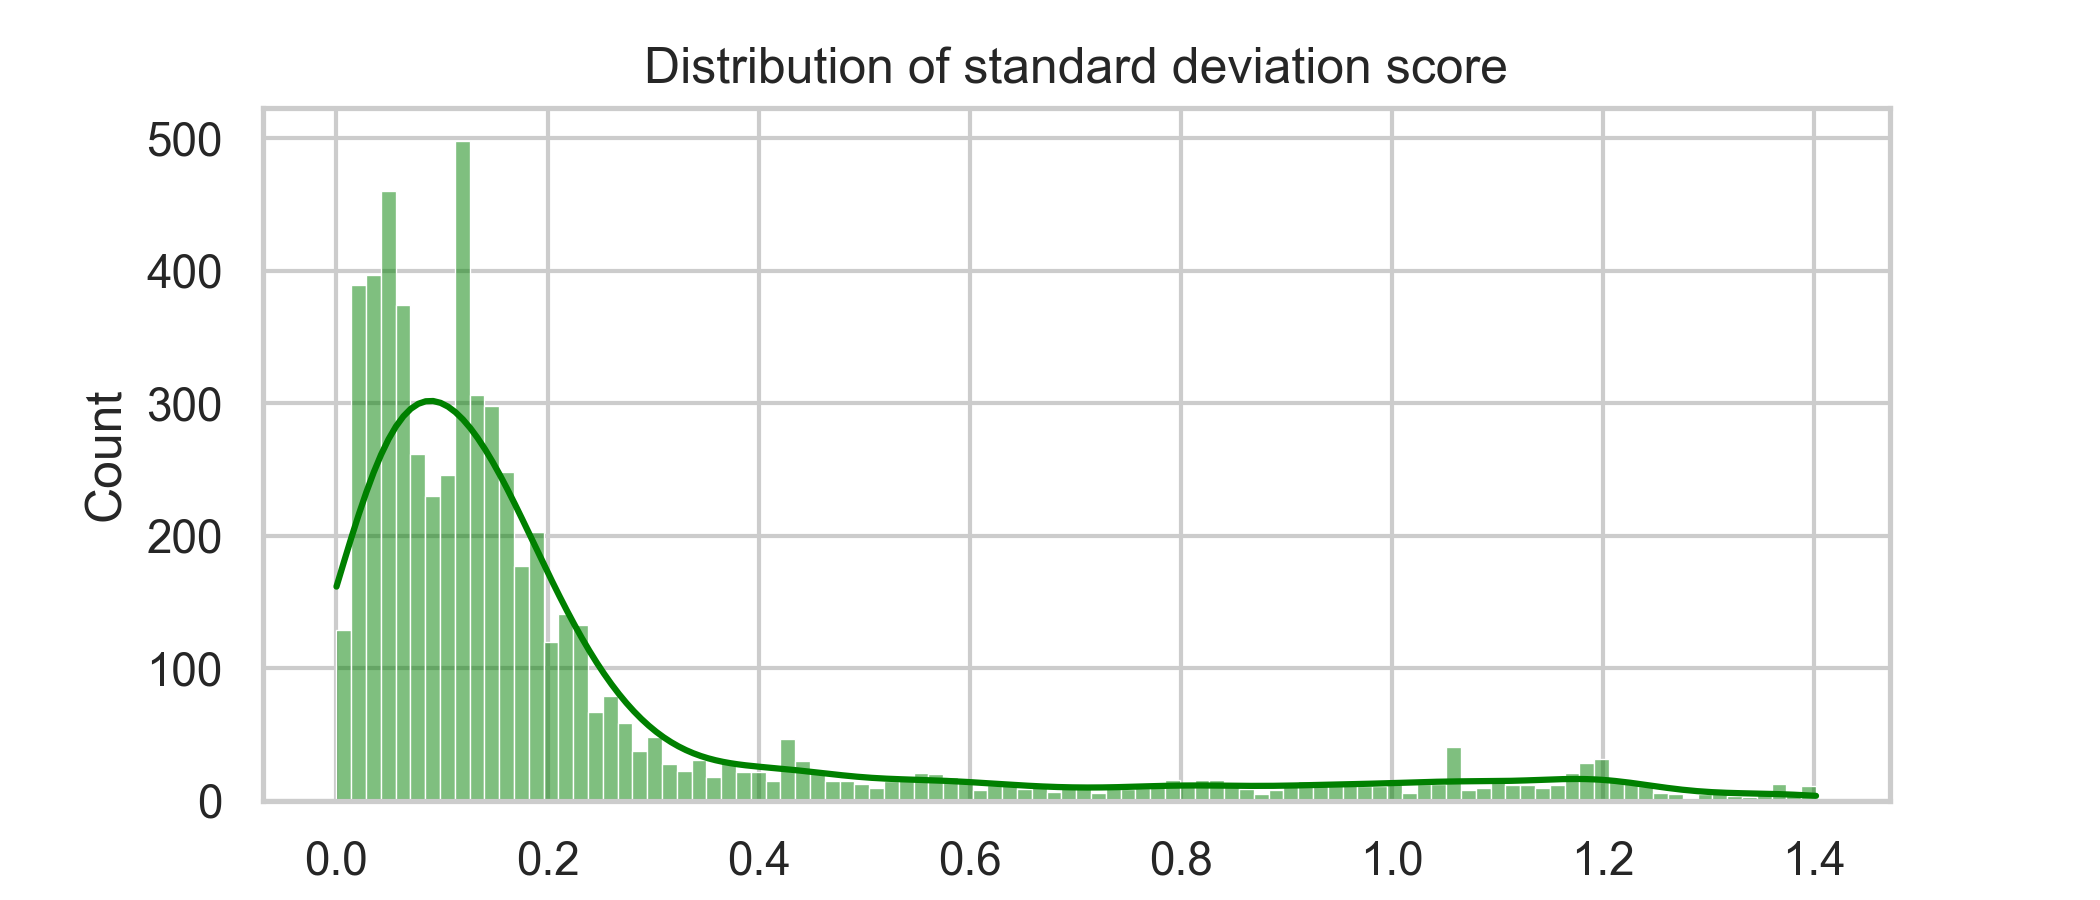
\includegraphics[width=0.9\linewidth]{Chapter5//figures/std_score.png}
    \caption{Enter Caption}
    \label{fig:std_avg}
\end{figure}



\section{RQ4 Polarization of experts vs know-it-all }
Out of the 22k users 16k are present only in one topics, 6k in more then one of which 3k only in 2 topics. \ref{fig:monopoli} do not show a difference in the ideology score between mono and poli user, to compute it we had to get the abs of the ideology so we do not have the problem of getting some mean around 0 

\begin{figure}
    \centering
    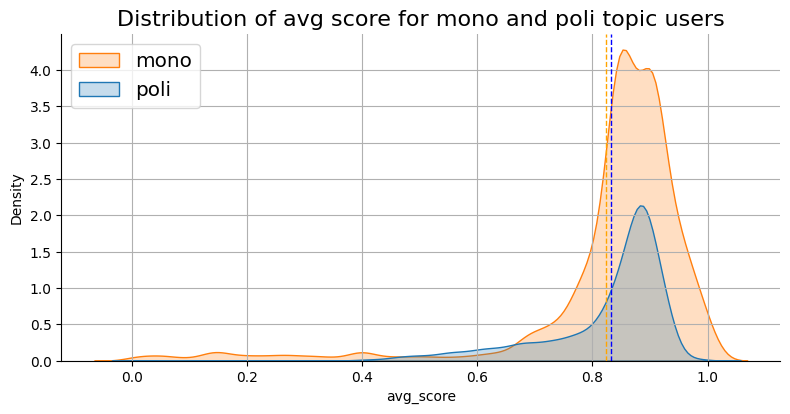
\includegraphics[width=0.8\linewidth]{Chapter5//figures/monopoli_score.png}
    \caption{Enter Caption}
    \label{fig:monopoli}
\end{figure}

